\documentclass[spanish]{beamer}


% esto me setea la variable pdf dependiendo del valor de \pdfoutput, que es >0
% sólo cuando estoy usando pdflatex para compilar el documento
\newif\ifpdf
\ifnum\pdfoutput<0
\pdffalse\fi
\ifnum\pdfoutput=0
\pdffalse\fi
\ifnum\pdfoutput>0
\pdftrue\fi

%\makeatletter
%\def\markboth#1#2{\def\leftmark{\@IEEEcompsoconly{\sffamily}\MakeUppercase{\protect#1}}%
%\def\rightmark{\@IEEEcompsoconly{\sffamily}\MakeUppercase{\protect#2}}}
%\makeatother


%
% ===
% === I18n / L10n
% ===
%
% babel me da separación de sílabas para palabras en el idioma que le paso como
%       argumento opcional. <-- Éste hay que pasarlo en \documentclass
%\usepackage{babel}
%
% inputenc define la codificación de caracteres del código fuente, acá utf8.
\usepackage[utf8]{inputenc}
%
% ===
% === Gráficos
% ===
% 
% pst-pdf me permite usar PSTricks con pdflatex. Necesito cargarlo sólo si está
%         definida la variable pdf, por eso está entre \ifpdf ... \fi
\ifpdf\usepackage{pst-pdf}\fi
%
% color me permite usar colores en el documento.
\usepackage{color}
%
% graphicx me da el comando \includegraphics para insertar imágenes (?)
\usepackage{graphicx}
%
% pstricks es un conjunto de macros basadas en PostScript para TeX, en
%          castellano, me da un entorno pstricks y comandos que uso dentro de
%          éste, que me sirven para dibujar figuras/diagramas/etc de manera
%          relativamente simple.
%\usepackage{pstricks}
%
% pst-circ me da macros para pstricks que me dibujan elementos de circuitos
%\usepackage{pst-circ}
%
% 
%\usepackage{pst-plot}		%Para dibujar una curva a partir de un archivo
%\usepackage{pst-2dplot}		%Para plotear. entorno pstaxes
%
% ===
% === Verbatims
% ===
%
% verbatim es una reimplementación de los entornos verbatim[*]
%          provee el comando \verbatiminput{archivo} y el entorno comment, que
%          hace que LaTeX ignore directamente todo lo que está adentro
%\usepackage{verbatim}
%
% moreverb implementa el entorno verbatimtab indentando los tabs que encuentre,
%          y también el entorno listing, que pone números de línea al verbatim.
%          Para cambiar el ancho de la tabulacion, uso
%          \renewcommand\verbatimtabsize{<ancho del tab>\relax}
%          También define el entorno boxedverbatim.
%\usepackage{moreverb}
%
% listings me da el entorno lstlisting con resaltado de sintaxis.
%          Para setear el lenguaje del código, hago \lstset{language=<lang>}
%\usepackage{listings}
%
% url es un verbatim para escribir URL's que permite linebreaks dentro de ésta.
%     para usarlo, \url{<URL>}
\usepackage{url}
%
%
%
%
%
%\usepackage{mdwlist}		%Para listas mas compactas
%\usepackage{textcomp}		%Para algunos símbolos
%\usepackage{colortbl}		%Para celdas de colores en tablas
%\usepackage{fancyhdr}		%Para encabezados/pie
%\usepackage{bbold}		%Fuente bb para modo math: \mathbb{R} = reales
%\usepackage{dsfont}		%Fuente ds para modo math: \mathds{R} = reales
\usepackage{multirow}		%Para "combinar" celdas en tablas
%\usepackage{float}		%Para cuadros, figuras, etc copadas
%\usepackage{fancybox}		%Para recuardos de texto con bordes "fancy"
%\usepackage{dingbat}		%Para dingbats
%%\usepackage{marginal}		%Para notas al margen que no puedo hacer andar
\usepackage{amsmath}		%Para enornos matemáticos mas flexibles
%\usepackage{varwidth}		%varwidth es un minipage que se ajusta al ancho mínimo
\usepackage{pslatex}            % setea fuentes Times, Helvetica y Courier ``angosta''

\usepackage[normalem]{ulem}     %para under/overlining. normalem hace que \emph se comporte como siempre


%Estilos de texto
\newcommand{\resalt}{\colorbox{green}}	%Resaltado - Fondo verde
\newcommand{\sfbf}{\bfseries\textsf}	%Slanted + Bold
\newcommand{\eng}{\textit}			%Palabra en inglés - Itálica
\newcommand{\mean}{\textsl}			%Significado de una sigla - Slanted
\newcommand{\defin}{\textbf}			%Definición - Negrita
\newcommand{\R}{\mathds}			%Para escribir R de Reales, N de Nat
\newcommand{\N}{\mathbf}			%Para escribir R de Reales, N de Nat
\newcommand{\lil}[1]{\footnotesize #1}
\newcommand{\mono}[1]{{\tt #1}}         % Monoespaciado


%Símbolos
\newcommand{\y}{\wedge}			%Y (Lógica)
\newcommand{\ve}{\vee}			%O (Lógica)
\newcommand{\ent}{\supset}		%Entonces (Lógica)
\newcommand{\dimp}{\leftrightarrow}	%Doble implicativo, equivalencia (Lógica)
\newcommand{\sii}{\leftrightarrow}	%Si y sólo si (Lógica)
\newcommand{\equi}{\equiv}		%Equivalencia (Lógica)
\newcommand{\portanto}{\vdash}	%Por lo tanto (Lógica)
\newcommand{\por}{\cdot}		%Producto punto

%Configuraciones del documento
%\selectlanguage{spanish}		%Elijo idioma español

%Tweaks
%\setlength{\parindent}{0mm}		%Sangría de 1a. línea
%\setlength{\hoffset}{-5.4mm}		%
%\setlength{\voffset}{-5.4mm}		%
%\setlength{\topmargin}{0mm}		%
%\setlength{\oddsidemargin}{5mm}	%
%\setlength{\evensidemargin}{5mm}	%
%\setlength{\marginparsep}{5mm}	%
%\setlength{\headheight}{12.5mm}	%
%\setlength{\headsep}{2.5mm}		%
%\setlength{\footskip}{10mm}		%
%\setlength{\textwidth}{15cm}		%
%\setlength{\textheight}{232mm}	%
%\setlength{\fboxrule}{.1pt}
%\setlength{\parskip}{.5\baselineskip}
%Colores
\definecolor{negro}	{cmyk}{0,0,0,1}
\definecolor{marron}	{cmyk}{0,.5,1,.41}
\definecolor{rojo}	{cmyk}{0,1,1,0}
\definecolor{naranja}	{cmyk}{0,.35,1,0}
\definecolor{amarillo}	{cmyk}{0,0,1,0}
\definecolor{verde}	{cmyk}{1,0,1,0}
\definecolor{azul}	{cmyk}{1,1,0,0}
\definecolor{violeta}	{cmyk}{.45,1,0,0}
\definecolor{gris}	{cmyk}{0,0,0,.5}
\definecolor{blanco}	{cmyk}{0,0,0,0}
\definecolor{dorado}	{cmyk}{0,.16,1,0}
\definecolor{plateado}	{cmyk}{0,0,0,.25}

%Comandos personalizados
\newcommand{\T}{\textrm}%Para escribir texto común cuando en modo math

% Remarca un ``texto insertado'' en rojo. Necesita el backage color.
\newenvironment{ins}{\color{red}$>$}{$<$}
\newcommand{\iins}[1]{{\color{red}$>$#1$<$}}

% Tacha un texto. Depende del package ulem.
\newcommand{\tachar}{\sout}

% Tacha doble
\newcommand{\Tachar}[1]{\xout{\xout{#1}}}

%\newcommand{\}

%\begin{pspicture}
%\def\tierra(#1){%Para dibujar el símbolo de tierra en el entorno PSTricks
%	\rput(#1){
%		\psdot(0,0)
%		\psline(0,0)(0,-0.45)
%		\psline(-0.5,-0.45)(0.5,-0.45)
%		\psline(-0.35,-0.6)(0.35,-0.6)
%		\psline(-0.2,-0.75)(0.2,-0.75)
%	}%
%}
%\end{pspicture}

%\newcommand{\codigo}[2]{%Para generar un recuadro con código
%	%\setlength{\hrulewidth}{0.1pt}
%	\begin{flushleft}
%	\underline{#1}
%	\begin{tabular}{@{\quad}|l}
%		\begin{minipage}{.85\textwidth}\smallskip{#2}
%	\end{minipage}\end{tabular}\end{flushleft}%
%}

%\newcommand{\filecodigo}[1]{%Insertar código verbatim desde un archivo
%\codigo{#1}{\verbatiminput{#1}}}%Requiere el paquete verbatim
%\newcommand{\filecodigobis}[1]{{\verbatiminput{#1}}}%Requiere el paquete verbatim

%\newcommand{\grafico}[3][1]{%Para generar un plot de un archivo con coords.
%%\def\deequis=#1
%\begin{minipage}{0.5\textwidth}\begin{center}
%\begin{pspicture}(6,5)
%	\psgrid[subgriddiv=1,gridlabels=0pt,gridwidth=.1pt](1,3)(1,1)(6,5)
%	\psset{xunit=5cm,yunit=2cm}
%	\fileplot[linewidth=1pt,linecolor=blue,origin={0.2,1.5}]{#2}
%	\psset{xunit=1cm,yunit=1cm}
%	\psaxes[Dx=#1,dx=5,Oy=-1,Dy=1,dy=2]{-}(0.9,1)(6,5)
%	\rput(4,0.4){\textsl{#3}}
%\end{pspicture}\end{center}\end{minipage}}

%\newcommand{\aclaracion}[1]{%Dibuja un recuadrito aclaratorio
%\smallpencil\ \begin{minipage}{0.9\textwidth}
%\vspace*{6pt}{#1}\smallskip\end{minipage}}

%\newcommand{\consigna}[1]{%Consigna - Slanted
%\leftpointright\ \parbox[t]{0.9\textwidth}{\textsl{#1}\vspace{8pt}}}

%\newcommand{\pinterno}[2]{%Consigna - Slanted
%\left\langle #1 , #2 \right\rangle}

%\newcommand{\eqncode}[2]{%
%\begin{center}
%\begin{tabular}{l@{\hspace{0.5cm}}r}
%\begin{minipage}{.4\textwidth}
%\begin{equation*}
%#1
%\end{equation*}
%\end{minipage}
%&
%\fbox{\begin{minipage}{.4\textwidth}
%%\setlength{\parskip}{4mm}
%\filecodigobis{#2}
%\end{minipage}}
%\end{tabular}
%\end{center}
%}

%\newcommand{\eqncodeb}[2]{%
%\begin{center}\begin{tabular}{l@{\hspace{0.5cm}}r}
%\begin{minipage}{.4\textwidth}#1\end{minipage} &
%\fbox{\begin{minipage}{.4\textwidth}\filecodigobis{#2}\end{minipage}}
%\end{tabular}\end{center}}

%\newenvironment{matemcode}[1]{\newline
%\begin{tabular}{l@{\hspace{0.5cm}}r}
%\begin{minipage}{.4\textwidth}
%\parbox[t]{.4\textwidth}{\begin{equation*}#1\end{equation*}}\end{minipage}
%&\begin{Sbox}\begin{minipage}{.4\textwidth}}
%{\end{minipage}\end{Sbox}\fbox{\TheSbox}\end{tabular}\newline}

%\newenvironment{encuadrar}[1]{\begin{Sbox}\begin{varwidth}{#1\textwidth}}
%{\end{varwidth}\end{Sbox}\fbox{\TheSbox}}

%\newenvironment{enunciado}
%{\leftpointright\ \begin{varwidth}[t]{0.9\textwidth}\textsl}
%{\end{varwidth}\vspace{8pt}}

%\newenvironment{parboxenv}{\begin{Sbox}}
%{\end{Sbox}\parbox[t]{.9\textwidth}{\TheSbox}}

%\newenvironment{pvi}{\begin{equation*}\begin{cases}}
%{\end{cases}\end{equation*}}

% Escribe el texto que le paso como parámetro con letra de ancho fijo.
%\newcommand{\mono}[1]{{\tt #1}}

%\title{\titulo}
%\author{\autor}
%\date{\fecha}

%% si uso pdflatex, me setea las propiedades del pdf de salida
%\ifpdf\pdfinfo{/Title    (\tituloPDF)
%               /Author   (\autorPDF)
%               /Subject  (\asuntoPDF)
%               /Keywords (\clavesPDF)}\fi

\include{beamerconf}
%
%
%\usetheme{Antibes}
\usetheme{Warsaw}
\usecolortheme{orchid}
%
%
%
\title{Identificación de edificios y monumentos a partir de fotografías tomadas 
con dispositivos móviles}
\author{Esteban C. Fornal \and Christian N. Pfarher \and Mauro J. Torrez}
\date{\today}

\begin{document}
%
\frame{\titlepage}

%%%%%%%%%%%%%%%%%%%%%%%%%%%%%%%%%%%%%%%%%%%%%%%%%%%%%%%%%
\section[Objetivo]{}

\begin{frame}{}
\frametitle{Objetivo}
Identificar edificios y monumentos a partir de fotografías
\end{frame}

%%%%%%%%%%%%%%%%%%%%%%%%%%%%%%%%%%%%%%%%%%%%%%%%%%%%%%%%%
\section[Herramientas utilizadas]{}

\begin{frame}{Herramientas}
\begin{itemize}
\item<1-> Transformada de Hough
\item<2-> Histograma
\end{itemize}
\end{frame}

%%%%%%%%%%%%%%%%%%%%%%%%%%%%%%%%%%%%%%%%%%%%%%%%%%%%%%%%%
\section[Técnicas utilizadas]{}
\subsection{Transformada de Hough}
\begin{frame}{Transformada de Hough}
\begin{center}  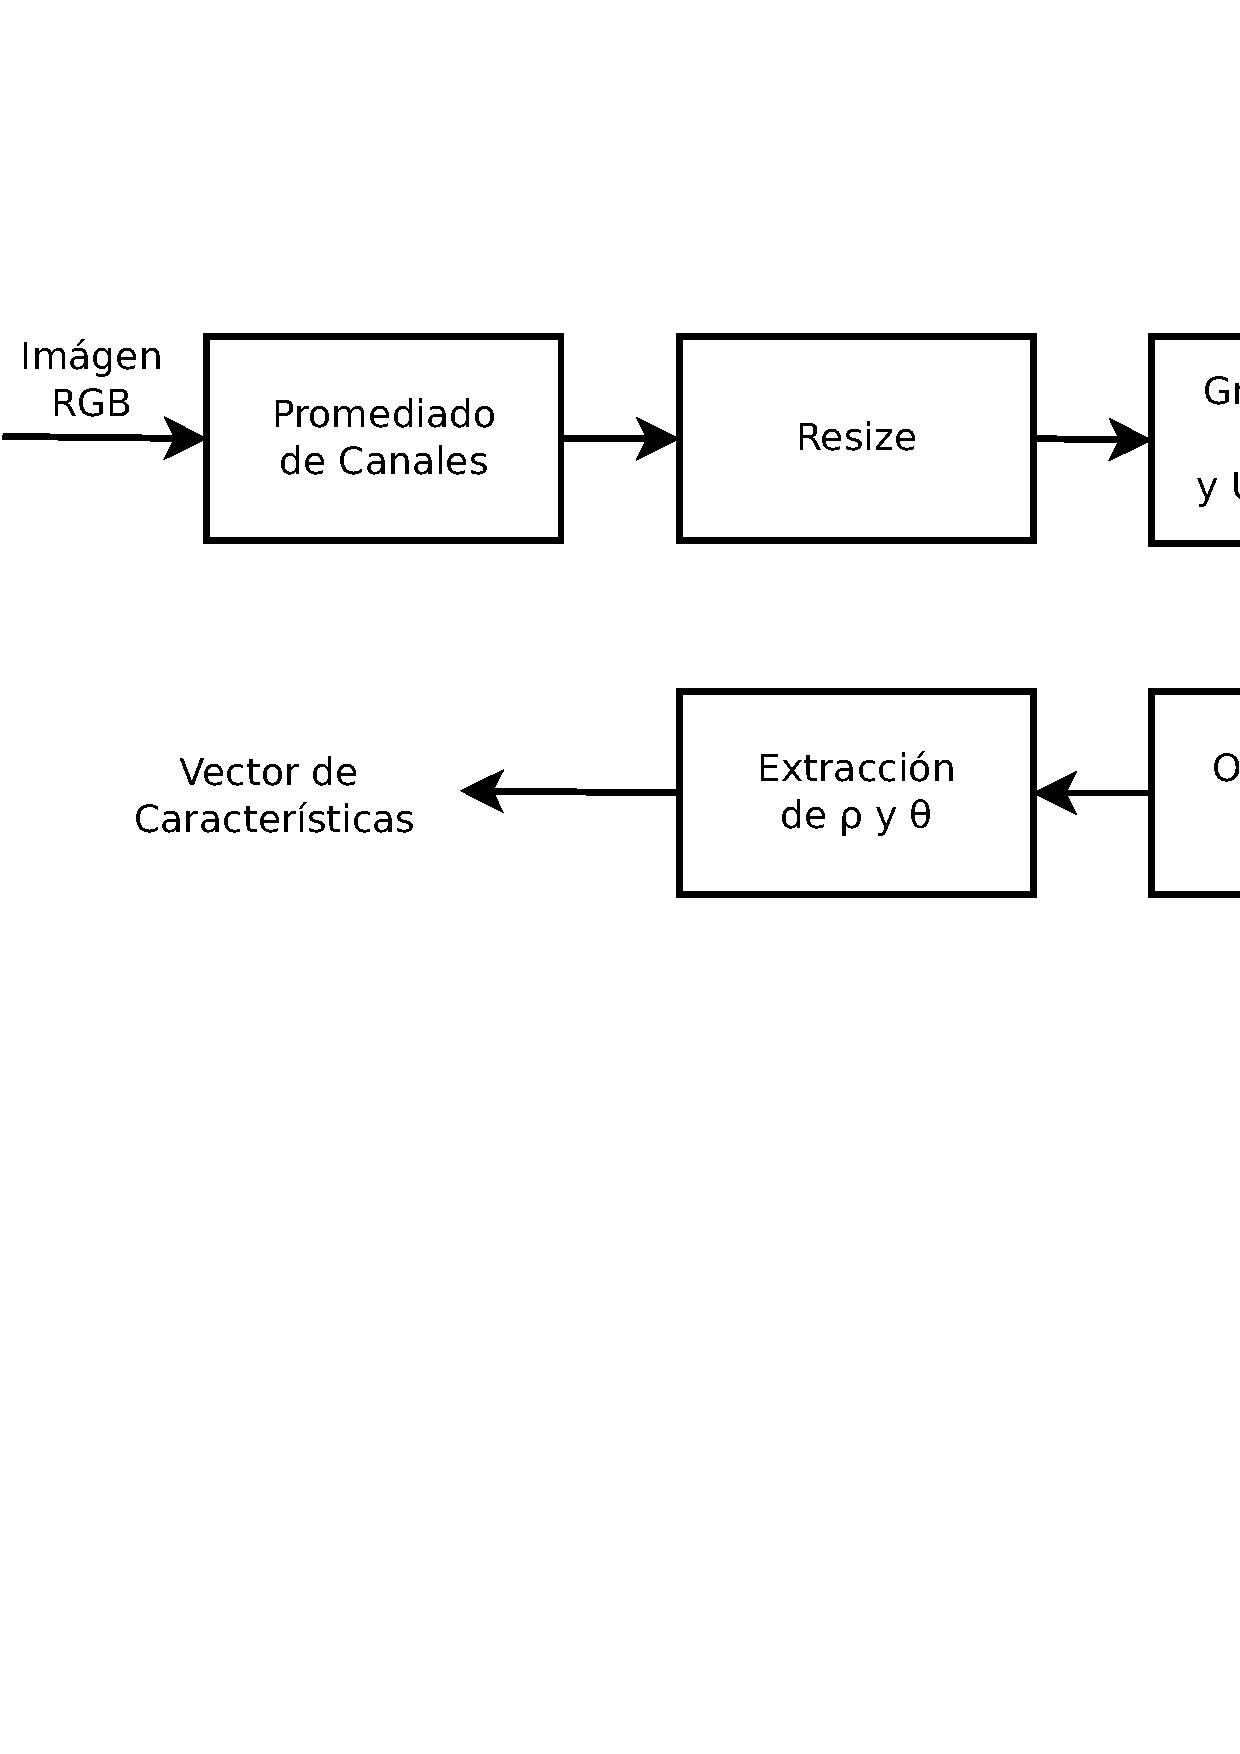
\includegraphics[width=9cm]{../diagramas/procesohough} \end{center}

  \begin{itemize}
  \item[]\begin{center}
    \begin{equation*}
      \label{umbral}
      f(I)=
      \begin{cases}
      0, & I\leq U\\
      255, & I > U
      \end{cases}
      \end{equation*}
      \end {center}
  \item 60 características
  \end{itemize}
\end{frame}
\subsection{Estadísticas del Histograma}
\begin{frame}{Estadísticas del Histograma}
 \begin{center} 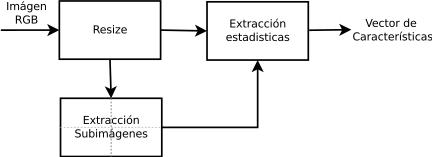
\includegraphics[width=9cm]{../diagramas/procesoestadisticas} \end{center}
  \begin{itemize}
  \item 45 características
  \end{itemize}
\end{frame}

%%%%%%%%%%%%%%%%%%%%%%%%%%%%%%%%%%%%%%%%%%%%%%%%%%%%%%%%%
\section[Método]{}
\subsection{Entrenamiento}
\begin{frame}{Entrenamiento}
  \begin{itemize}
  \item Etiquetado de imágenes
  \item Generación de prototipos
  \end{itemize}
\end{frame}
\subsection{Clasificación}
\begin{frame}{Clasificación}
  \begin{itemize}
  \item Error cuadrático medio
    \begin{align*}
      MSE = \frac{1}{MN} \sum_x\sum_y [ f(x,y) - g(x,y) ]^{2}
    \end{align*}
  \item Obtención de la Clase
  \end{itemize}
\end{frame}

%%%%%%%%%%%%%%%%%%%%%%%%%%%%%%%%%%%%%%%%%%%%%%%%%%%%%%%%%
\section[Pruebas]{}

\subsection{Armado Base de Datos}
\begin{frame}{Armado Base de Datos}
  \begin{itemize}
  \item Imágenes de 640x480
  \item Obtenidas con celular
  \item Diurnas y nocturnas
  \end{itemize}
\end{frame}

\subsection{Conjunto de Imágenes}
\begin{frame}{Clases}
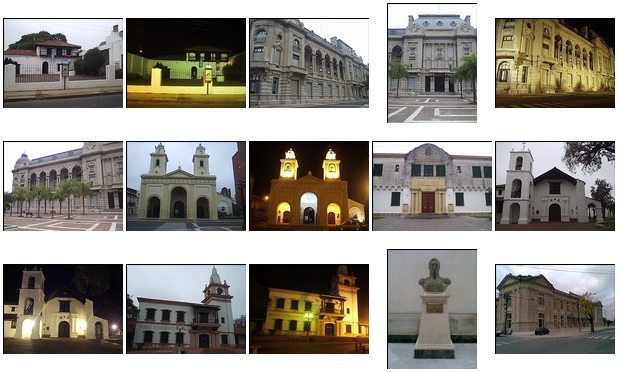
\includegraphics[width=10cm]{img/mosaico.png} 
\end{frame}

\begin{frame}{Imágenes de prueba}
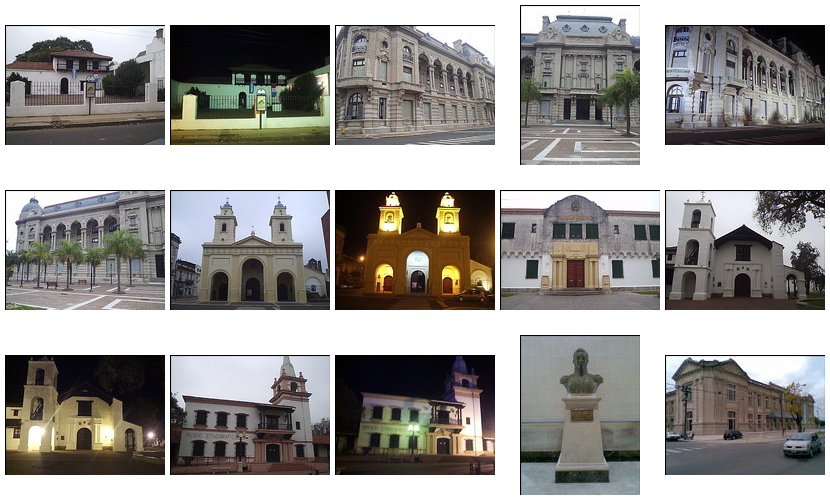
\includegraphics[width=10cm]{img/pruebas.png} 
\end{frame}

\subsection{Sólo con técnica de T. de Hough}
\begin{frame}{Sólo con la técnica de Hough}
Determinación de umbral y cantidad de máximos a utilizar
  \begin{center}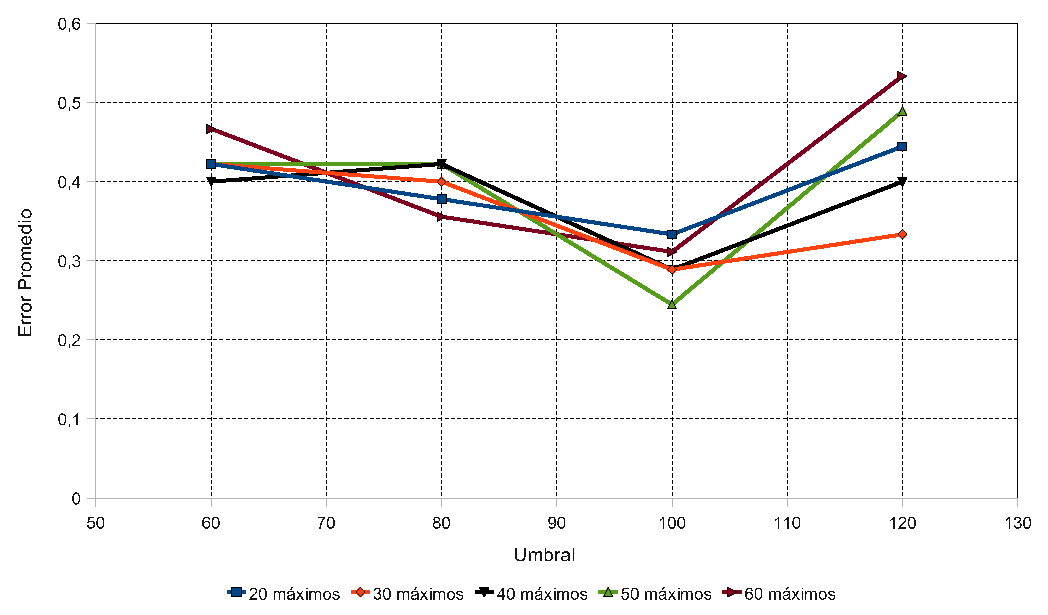
\includegraphics[width=9cm]{../diagramas/estadistica_noche_iguales} \end{center}
\end{frame}

\subsection{Sólo con técnica de histograma}
\begin{frame}{Sólo con la técnica de histograma}
\end{frame}

\subsection{Ambas técnicas}
\begin{frame}{Ambas técnicas}
  \begin{itemize}
  \item Igual ponderación
  \end{itemize}
\end{frame}

\subsection{Cómo se hicieron?}
\begin{frame}{Procedimiento}
  \begin{itemize}
  \item gráfica con generación prototipo de 5 imágenes la q hicimos en pizarrón
  \end{itemize}
\end{frame}

%%%%%%%%%%%%%%%%%%%%%%%%%%%%%%%%%%%%%%%%%%%%%%%%%%%%%%%%%
\section[Resultados]{}
\begin{frame}{Resultados}
  Se considera la tasa de error según:
  \begin{equation*}
    E_{\%}=100\cdot\frac{\T{número de errores}}{\T{número de pruebas}},
  \end{equation*}


  Tasas de error para las técnicas de extracción de características
  \begin{center}\begin{tabular}{ccc}
      \hline \emph{{Técnica}} & \emph{5 etiquetas} & \emph{15 etiquetas}\\
      \hline Histogramas & 0\% & 0\%\\
      \hline Hough & 35.5\% & 60.43\%\\
      \hline Ambas & 2.22\% & 4.17\%\\
      \hline
  \end{tabular}\end{center}
  \label{tablaerrores}


\end{frame}


%%%%%%%%%%%%%%%%%%%%%%%%%%%%%%%%%%%%%%%%%%%%%%%%%%%%%%%%%
\section[Conclusiones]{}

\begin{frame}{Conclusiones}
  \begin{itemize}
  \item Sensores
    \begin{itemize}
    \item Cantidad
    \item Tipo
    \item Configuración
    \end{itemize}
  \item Resultados satisfactorios para la información disponible
  \end{itemize}
\end{frame}

\end{document}